\documentclass[conference]{IEEEtran}
\IEEEoverridecommandlockouts

\usepackage{cite}
\usepackage{amsmath,amssymb}
\usepackage{graphicx}
\usepackage{textcomp}
\usepackage{xcolor}
\usepackage{url}
\usepackage{tikz}
\usetikzlibrary{shapes.geometric, arrows.meta, positioning}

\def\BibTeX{{\rm B\kern-.05em{\sc i\kern-.025em b}\kern-.08em
    T\kern-.1667em\lower.7ex\hbox{E}\kern-.125emX}}

\begin{document}

\title{IndicBridge: Investigating Linguistic Relatedness in\\
Cross-Lingual Multistage Fine-Tuning of Whisper for\\
Low-Resource Indic Speech Recognition}

\author{
\IEEEauthorblockN{Gourab Dash}
\IEEEauthorblockA{\textit{School of Computer Science and Engineering}\\
\textit{RV University}, Bengaluru, India\\
1RUA24CSE0146}
\and
\IEEEauthorblockN{Parth Nandkumar Khandagale}
\IEEEauthorblockA{\textit{School of Computer Science and Engineering}\\
\textit{RV University}, Bengaluru, India\\
1RUA24CSE0201}
\and
\IEEEauthorblockN{Divyansh Mahecha}
\IEEEauthorblockA{\textit{School of Computer Science and Engineering}\\
\textit{RV University}, Bengaluru, India\\
1RUA24CSE0139}
\and
\IEEEauthorblockN{Kaushal BC}
\IEEEauthorblockA{\textit{School of Computer Science and Engineering}\\
\textit{RV University}, Bengaluru, India\\
1RUA24CSE0196}
}

\maketitle

\begin{abstract}
Speech recognition has improved considerably, but the improvement has not reached all languages equally. For several Indian languages, limited transcribed data and uneven representation in pre-trained models still make reliable recognition difficult. This paper presents IndicBridge, a study of whether an intermediate language helps Whisper adapt to a low-resource target. We use Whisper-base with Low-Rank Adaptation (LoRA) and compare direct fine-tuning with two-stage training through Hindi or English. Marathi, Odia and Kannada are the target languages; evaluation uses FLEURS and Kathbath. With the Hindi pivot, WER falls by 3.1 and 3.5 points for Marathi, 3.1 and 1.9 for Odia, and 1.1 and 0.8 for Kannada across the two test sets. An equally sized English pivot gives no significant positive gain. We also examine Odia's tokenizer and decoder limits, borrowed language tokens, normalization choices and offline deployment. The results show that pivot selection matters in this setting, but they do not establish language-family membership as the sole reason for the improvement. The work comprises 25 runs carried out on one Apple M4 machine.
\end{abstract}

\begin{IEEEkeywords}
Automatic Speech Recognition, Low-Resource Languages, Cross-Lingual
Transfer, Multistage Fine-Tuning, Whisper, LoRA, Parameter-Efficient
Fine-Tuning, Indic Languages, Odia, Word Error Rate.
\end{IEEEkeywords}

% ======================================================================
\section{Introduction}

\subsection{Background and Context}

Speech recognition systems were traditionally built for individual
languages and depended on large collections of accurately transcribed
audio. This approach worked well for languages with established digital
resources, but it left many others with limited or no practical support.
The use of multilingual pre-training changed this situation. Models such
as wav2vec 2.0, XLSR-53 and XLS-R showed that speech representations
learned from several languages can be reused when adapting a model to a
particular language with less labelled data \cite{conneau2021xlsr,babu2022xlsr}.

Whisper followed a different route. It was trained on a large collection
of weakly labelled multilingual audio and uses one encoder--decoder
Transformer for tasks such as transcription, translation and language
identification \cite{radford2023whisper}. This scale gives Whisper useful
zero-shot ability for languages that are well represented in its training
data. It does not, however, mean that every supported language receives
the same level of performance. Recognition quality varies across the
language set, and languages with less training data often need further
adaptation. Massively Multilingual Speech (MMS) took language coverage
even further, reporting speech technology for more than one thousand
languages \cite{pratap2024mms}.

For Indian languages, the gap between nominal support and useful
recognition is still important. A model may be able to produce text in a
script without reliably recognizing the speech behind it. The available
training data, the language token used during decoding and the way the
output is evaluated can all affect the result. These issues are central
to the present study.

\subsection{Motivation and Research Gap}

IndicBridge began with a question raised by earlier work on multistage
fine-tuning. Pillai \emph{et al.}\ reported an improvement when Whisper
was adapted to Malasar through Tamil, and discussed the relationship
between the two Dravidian languages as a possible reason for the result
\cite{pillai2026multistage}. The result is useful, but it leaves an open
question: would a more distant, non-Indic intermediate language have helped as well
if it had supplied the same amount of speech and training? A second
concern was that a smaller gain for Kannada might simply reflect the
difficulty of that target. We therefore needed a control pivot for each
target, not just a comparison between the two target families.

Earlier studies give reasons to consider linguistic similarity, but they
do not isolate it from other factors. Rouditchenko \emph{et al.}\ found
that pre-training exposure at both language and family levels helps
predict adaptation to unseen languages \cite{rouditchenko2023unseen}.
Song \emph{et al.}\ also explored language similarity when extending
multilingual ASR with LoRA \cite{song2024lorawhisper}. The experiments
reported in those studies do not provide the matched pivot comparison
needed to answer our question directly. We therefore compare Hindi and
English pivots with the same audio duration and training-step budget,
then adapt each model to Marathi, Odia or Kannada.

% ======================================================================
\section{Literature Review}

\subsection{Multilingual Speech Representation Learning}

Conneau \emph{et al.}\ introduced XLSR-53, which extended wav2vec 2.0 to
self-supervised pre-training over 53 languages. Their results showed that
multilingual speech representations can be useful when adapting to
individual low-resource languages \cite{conneau2021xlsr}. XLS-R later
expanded the approach to 128 languages and models of up to two billion
parameters, reporting improvements across speech recognition and related
tasks \cite{babu2022xlsr}. They do not, however, give a simple answer to
which source language is the best choice for a particular target.

\subsection{Weakly-Supervised Multilingual ASR}

Whisper is based on large-scale weak supervision rather than a separate
self-supervised stage followed by language-specific training. Its
training data contains audio paired with noisy or loosely prepared text,
and the resulting model performs well in a zero-shot setting for many
well-represented languages \cite{radford2023whisper}. Whisper uses a
fixed inventory of language tokens to guide decoding. Hindi, Bengali,
Assamese, Marathi and Kannada are included in this inventory, but Odia
has no dedicated token. The byte-level tokenizer can still encode Odia
characters, although it uses more tokens to represent them. This makes
Odia a useful case for examining both the effect of a borrowed language
token and the practical limits of the decoder.

\subsection{Adaptation to Languages Unseen During Pre-Training}

Rouditchenko \emph{et al.}\ compared XLS-R and Whisper on languages that
were both seen and unseen during pre-training. They found that the amount
of pre-training exposure at the language and language-family levels was
useful in predicting how well a model adapted \cite{rouditchenko2023unseen}.
However, their analysis considered previous pre-training exposure. It
did not directly change the intermediate language used in a controlled
fine-tuning pipeline.

\subsection{Sequential and Multistage Transfer}

Pillai \emph{et al.}\ studied multistage fine-tuning for Malasar, a very low-resource Dravidian language. They first adapted Whisper using Tamil speech and then fine-tuned it for Malasar. Their reported WER was 51.9\%, which was 4.5 points lower than direct fine-tuning; removing punctuation reduced it further to 47.3\% \cite{pillai2026multistage}. At that very time, it also evaluates only one pivot--target pair. Without a comparison against a distant or a non-Indic pivot, it isn't possible to tell how much of the gain comes specifically from the relationship between Tamil and Malasar.

\subsection{Parameter-Efficient Adaptation}

LoRA reduces the number of parameters that need to be updated during
fine-tuning by representing the weight change with low-rank matrices
\cite{hu2022lora}. For speech recognition, Song \emph{et al.}\ introduced
LoRA-Whisper for multilingual ASR and explored how language similarity
can be used when adding languages to a model \cite{song2024lorawhisper}.
Xu \emph{et al.}\ examined LoRA-based multilingual extension without
rehearsal data \cite{xu2024rehearsalfree}, while Ferraz \emph{et al.}\
used language-specific experts in a smaller distilled model
\cite{ferraz2024distilwhisper}. Earlier adapter work
\cite{houlsby2019adapters,pfeiffer2020madx} applied the same idea to
text models.

\subsection{Indic Speech Resources and Systems}

AI4Bharat has released several resources for Indian language speech.
IndicVoices contains natural and spontaneous recordings from speakers
across many regions and languages \cite{javed2024indicvoices}. The
IndicSUPERB benchmark introduced Kathbath as part of an evaluation suite
for Indian speech processing \cite{javed2023indicsuperb}.

Bhogale \emph{et al.}\ presented Vistaar, a collection of benchmarks covering different Indian languages and domains, and trained IndicWhisper on multilingual Indian speech \cite{bhogale2023vistaar}. Their results also show that model rankings can change across benchmarks. This is one reason our evaluation uses both FLEURS and Kathbath instead of relying on a single test set. FLEURS provides parallel speech across many languages \cite{conneau2023fleurs}, whereas Kathbath provides the Indian language evaluation resource \cite{javed2023indicsuperb}. IndicWhisper uses joint multilingual training, whereas our work studies sequential pivot-to-target adaptation.

\subsection{Comparative Analysis}

Table~\ref{tab:comparison} will summarize the studies as discussed above, together with the limitation most relevant to the IndicBridge research questions.

\begin{table*}[!t]
\caption{Comparative Analysis of the Reviewed Studies}
\label{tab:comparison}
\centering
\renewcommand{\arraystretch}{1.15}
\scriptsize
\begin{tabular}{|p{2.5cm}|p{4.2cm}|p{4.9cm}|p{4.9cm}|}
\hline
\textbf{Study} & \textbf{Method / Model} &
\textbf{Key Finding} & \textbf{Key Limitation} \\
\hline
Conneau \emph{et al.} \cite{conneau2021xlsr} &
XLSR-53, cross-lingual wav2vec 2.0 &
Shared cross-lingual representations outperform monolingual pre-training. &
Transfer studied in aggregate; no pairwise source--target analysis. \\
\hline
Babu \emph{et al.} \cite{babu2022xlsr} &
XLS-R, up to 2B parameters, 128 languages &
Scaling cross-lingual self-supervision improves low-resource ASR. &
Very large compute requirement; family effects not isolated. \\
\hline
Radford \emph{et al.} \cite{radford2023whisper} &
Whisper, weakly-supervised encoder--decoder (680K hours) &
Large-scale weak supervision yields robust zero-shot ASR. &
Closed 99-language token set; Odia absent; highly uneven per-language quality. \\
\hline
Pratap \emph{et al.} \cite{pratap2024mms} &
MMS, 1000+ language ASR &
Language coverage can be extended by an order of magnitude. &
Supervision drawn from a narrow domain; limited generality. \\
\hline
Rouditchenko \emph{et al.} \cite{rouditchenko2023unseen} &
Fine-tuning XLS-R vs.\ Whisper (13 unseen, 18 seen languages) &
Pre-training hours per language and per family predict adaptation quality. &
Family exposure is observational, not experimentally manipulated. \\
\hline
Pillai \emph{et al.} \cite{pillai2026multistage} &
Multistage fine-tuning, Whisper via Tamil pivot (Malasar, $\approx$4h36m) &
51.9\% WER, 4.5\% absolute gain over direct fine-tuning; 47.3\% after punctuation removal. &
Single pivot--target pair; relatedness claim not tested against a distant-language control. \\
\hline
Hu \emph{et al.} \cite{hu2022lora} &
LoRA low-rank adaptation &
Comparable quality while training under 1\% of parameters. &
Not originally evaluated for speech or cross-lingual transfer. \\
\hline
Song \emph{et al.} \cite{song2024lorawhisper} &
LoRA-Whisper for multilingual ASR &
Mitigates language interference; language similarity aids new-language extension. &
Similarity exploited heuristically, not measured as an independent variable. \\
\hline
Ferraz \emph{et al.} \cite{ferraz2024distilwhisper} &
DistilWhisper with language-specific experts &
Distillation retains per-language capability at reduced size. &
Compression-oriented; no pivot-language analysis. \\
\hline
Bhogale \emph{et al.} \cite{bhogale2023vistaar} &
Vistaar benchmarks; IndicWhisper (59 benchmarks, 12 languages, 10.7K hours) &
Lowest WER on 39/59 benchmarks; rankings vary across benchmarks. &
Joint multilingual training; pairwise transfer not isolated. \\
\hline
Javed \emph{et al.} \cite{javed2024indicvoices} &
IndicVoices corpus (23.7K hours, 51K speakers, 22 languages) &
Large-scale spontaneous Indian speech resource. &
Dataset contribution; no transfer-strategy study. \\
\hline
Javed \emph{et al.} \cite{javed2023indicsuperb} &
IndicSUPERB / Kathbath &
Standardized evaluation across Indian languages. &
Benchmark rather than adaptation methodology. \\
\hline
Pi\~{n}eiro-Mart\'{i}n \emph{et al.} \cite{pineiro2024weighted} &
Weighted cross-entropy for imbalanced multilingual ASR &
Objective reweighting improves low-resource languages. &
Addresses optimization, not evaluation normalization. \\
\hline
\end{tabular}
\end{table*}

% ======================================================================
\section{Identified Gaps and Proposed Direction}

\subsection{Gaps in the Literature}

There are three gaps that are relevant to this work. At first, multistage fine-tuning has been shown to help low-resource ASR, and previous research had linked transfer quality to language-family exposure. What was not tested directly is whether a related pivot performs better than a more distant, non-Indic one when the audio hours and training schedule are matched.

Second, languages without a dedicated token in the pre-trained model need more attention. Odia is a useful test case because Whisper can represent its script but doesn't provide an Odia language token. Therefore, it is necessary to examine if borrowing a token from another language affects recognition, both before and after fine-tuning.

Third, the evaluation across Indic scripts needs some care.

\subsection{Research Questions}

The main question addressed in this paper is:

\begin{quote}
\textbf{Does multistage cross-lingual fine-tuning work better because
the pivot language is related to the target, or can the same improvement
be obtained simply by adding an equal amount of pivot-language data?}
\end{quote}

We also examine three related questions:

\begin{enumerate}
    \item Does the Hindi pivot provide a different level of improvement
    for the Indo-Aryan targets Marathi and Odia than it does for the
    Dravidian target Kannada, when the training budget is matched?
    \item For Odia, which of the available borrowed language tokens---
    Bengali, Assamese or Hindi---gives the best recognition result, and
    does the observed ranking follow linguistic proximity?
    \item How much do text-normalization choices change WER and CER for
    Indic scripts, and can they also change the ranking of the compared
    adaptation methods?
\end{enumerate}

\subsection{Proposed Direction}

IndicBridge addresses these questions through a controlled set of experiments using Whisper-base. Hindi is used as the Indic pivot and English as a distant, non-Indic control. We keep the model and the optimizer and decoding setup and scoring procedure consistent and accurate across every single run.

% ======================================================================
\section{Problem Statement}

Adapting a multilingual speech model to a low-resource language is not simply a matter of adding a few more training steps. A small target corpus may not contain enough examples for the model to learn the language's pronunciation, vocabulary and writing conventions. One of the possible responses is adapting the model first on an intermediate language and then continuing the training on the target. What remains a question is why this extra stage helps. The pivot may share useful properties with the target, or the model may benefit simply from seeing more speech before target-language training.

That distinction affects how a pivot should be chosen. A practitioner might look for a related language or might choose whichever language has the largest available corpus. Earlier work reported an improvement for Tamil-to-Malasar adaptation but did not include a distant-language control pivot \cite{pillai2026multistage}. The aim is to test if Hindi provides an advantage over an equal duration of English pivot, not to assume in advance that language family alone explains any gain.

% ======================================================================
\section{Methodology}

\subsection{Experimental Design}

The experimental pipeline is shown in Fig.~\ref{fig:arch}. Direct fine-tuning was the reference condition and had started from a fresh LoRA adapter rather than the one learned on a pivot.

There were 25 runs in total: six zero-shot configurations, two pivot training runs, six pivot-only evaluations, three direct target runs, three Hindi-to-target runs, three English-to-target runs and two extra Odia-token runs. Bengali was selected as the default borrowed token before any results were examined; Assamese and Hindi were added as ablations rather than being chosen after seeing which one scored best. We also used a simple gate before starting the target-language grid: the Hindi pivot had to improve on zero-shot Hindi first. It did, reducing WER from 154.7 to 41.0 on FLEURS and from 137.0 to 44.0 on Kathbath. A resumable queue runs the jobs one after another on the M4, records failures and continues after a crash or sleep.

\begin{figure}[!t]
\centering
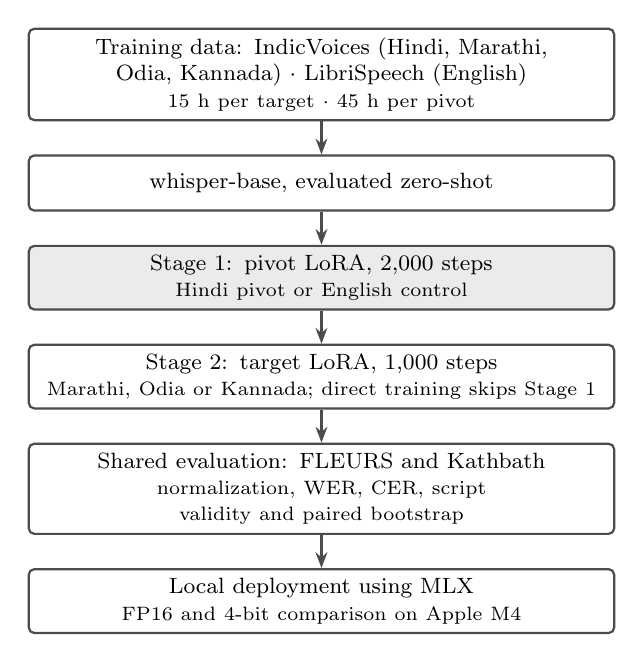
\begin{tikzpicture}[
  node distance=4.2mm,
  box/.style={rectangle, rounded corners=2pt, draw=black!70, thick,
              text width=7.2cm, align=center, minimum height=7mm,
              font=\footnotesize},
  ctrl/.style={box, fill=black!8},
  arrow/.style={-{Stealth[length=2mm]}, thick, draw=black!70}
]
\node[box] (data) {Training data: IndicVoices (Hindi, Marathi, Odia, Kannada) $\cdot$ LibriSpeech (English)\\ \scriptsize 15 h per target $\cdot$ 45 h per pivot};
\node[box, below=of data] (base) {whisper-base, evaluated zero-shot};
\node[ctrl, below=of base] (pivot) {Stage 1: pivot LoRA, 2,000 steps\\ \scriptsize Hindi pivot or English control};
\node[box, below=of pivot] (stage2) {Stage 2: target LoRA, 1,000 steps\\ \scriptsize Marathi, Odia or Kannada; direct training skips Stage 1};
\node[box, below=of stage2] (eval) {Shared evaluation: FLEURS and Kathbath\\ \scriptsize normalization, WER, CER, script validity and paired bootstrap};
\node[box, below=of eval] (deploy) {Local deployment using MLX\\ \scriptsize FP16 and 4-bit comparison on Apple M4};
\draw[arrow] (data) -- (base);
\draw[arrow] (base) -- (pivot);
\draw[arrow] (pivot) -- (stage2);
\draw[arrow] (stage2) -- (eval);
\draw[arrow] (eval) -- (deploy);
\end{tikzpicture}
\caption{Overview of the IndicBridge pipeline. The intermediate stage
uses Hindi, English or no pivot; the target-language stage is kept the
same across the corresponding comparisons.}
\label{fig:arch}
\end{figure}

% Generated by report/paper/build_assets.py from results/. Do not edit numbers by hand.
\begin{table}[!t]
\caption{Experimental Setup, Identical for Every Run}
\label{tab:setup}
\centering\scriptsize
\renewcommand{\arraystretch}{1.12}
\begin{tabular}{@{}p{1.55cm}p{6.35cm}@{}}
\hline
Base model & whisper-base (74M parameters), frozen\\
LoRA & $r{=}32$, $\alpha{=}64$, dropout 0.05, on $W_q$, $W_v$; 1.18M trainable\\
Optimiser & AdamW, lr $10^{-3}$, 100 warm-up steps, linear decay, grad.\ clip 1.0\\
Batch / precision & effective batch 16, fp32, seed 42\\
Steps & pivot 2000, target 1000\\
Hindi pivot & IndicVoices, 45 h, 19,127 clips, 1,474 speakers\\
English pivot & LibriSpeech clean-100, 45 h, 12,895 clips, 124 speakers\\
Marathi target & IndicVoices, 15 h, 6,141 clips, 721 speakers\\
Odia target & IndicVoices, 15 h, 7,227 clips, 1,150 speakers\\
Kannada target & IndicVoices, 15 h, 6,335 clips, 720 speakers\\
Clip filters & 2--30 s; $\le$50 clips per speaker; tagged rows dropped; labels $\le$443 tokens\\
Test sets & FLEURS test, Kathbath valid: 600 seeded clips each (Hindi FLEURS: all 417)\\
Decoding & greedy, no repetition penalty, length cap per language\\
Hardware & Apple M4, 16 GB unified memory, PyTorch (MPS)\\
\hline
\end{tabular}
\end{table}


\subsection{Data}

Hindi, Marathi, Odia and Kannada training audio came from IndicVoices
\cite{javed2024indicvoices}; English came from the LibriSpeech
clean-100 subset \cite{panayotov2015librispeech}. The IndicVoices
archives were too large to download in full (roughly 36--59 GB per
language), so we sampled data shards spread across the collection using
a fixed seed. Duration metadata was checked before decoding the audio.

We removed clips shorter than two seconds or longer than 30 seconds, as well as rows containing annotation tags such as \texttt{<unintelligible>}. The tag filter did the job by removing 1,044 Hindi rows, 704 Odia rows, 285 Kannada rows and 157 Marathi rows. We limited the Indian-language training data to 50 clips per speaker; English used a limit of 120 because its speakers had longer recordings. Whisper's decoder has a 448-token context limit, so the training labels were capped at 443 tokens to leave space for the task and language special tokens. This removed 1,076 Odia clips and 158 Kannada clips.

The test data was kept separate from training. We used the FLEURS test
split \cite{conneau2023fleurs} and the Kathbath validation split
\cite{javed2023indicsuperb}, taking a fixed seeded sample of 600 clips
where available; all 417 Hindi FLEURS clips were used. Common Voice
\cite{ardila2020commonvoice} had been the planned alternative, but its
Hugging Face entry exposed only a README by the time of the experiments.
References longer than 440 tokens were excluded because the decoder
could not emit the complete transcript. This affected 202 of 875 Odia
FLEURS references (23.1\%) and 11 of 831 Kannada references (1.3\%); no
references were excluded in the other language/test-set combinations.

\subsection{Model and Training}

We used the 74-million-parameter Whisper-base model as the starting
point \cite{radford2023whisper}. Its original weights were kept frozen, and
LoRA adapters \cite{hu2022lora} were added to the query and value
projections in each attention block, using Hugging Face Transformers
\cite{wolf2020transformers} and PEFT \cite{peft2022}. The rank was 32
and the scaling parameter $\alpha$ was 64. This left approximately 1.18
million trainable parameters, or 1.6\% of the model. The update is
written as
\begin{equation}
W = W_0 + \frac{\alpha}{r}BA, \qquad
B \in \mathbb{R}^{d\times r},\quad A \in \mathbb{R}^{r\times k},
\label{eq:lora}
\end{equation}
where $W_0$ is frozen and $A$ and $B$ are the learned low-rank matrices.

In multistage runs, target training continued from the pivot adapter, and the direct runs began with a fresh adapter; the remaining settings are listed in Table~\ref{tab:setup}. We chose Whisper-base for a practical reason. On the M4, Whisper-small trained at a rate of 1.35 clips/s, which put the grid near 49 hours at the step budget used here. Whisper-base reached about 4.54 clips/s, which brought the estimate to roughly 15 hours. The absolute WER of base is consequently higher than it would be with a larger model.

The only real problem is memory usage, and we have put a limit on the MPS allocation at around 9.5 GB so that the machine does not start swapping heavily. Variable label lengths caused out-of-memory errors twice in the Hindi pivot, because MPS cached a separate computation graph for each label length. The labels were padded to multiples of 64, leading to seven different shapes. The micro-batch/accumulation layout was changed from 4-by-4 to 2-by-8, but the effective batch of 16 remained the same.

\subsection{Odia and the Borrowed Language Token}

Whisper does not include an Odia language token, so Odia decoding had
to use a token from another language. We fixed Bengali as the default
before running the experiments because it was the closest available
relative in the tokenizer inventory. Assamese and Hindi were then tested
as ablations. Script validity was measured as the percentage of
generated letters that belong to the target language's Unicode script
block, because a model can produce a phonetic rendering of speech and
still write it in the wrong script.

\subsection{Decoding, Normalization and Metrics}

Some of the decoding settings in our initial build plan did not work
for Odia. Its letters are often represented by several byte-level
tokens, so a repetition penalty can suppress sequences that are part of
normal spelling, and a 200-token output limit cut off Odia transcripts.
We therefore used plain greedy decoding, with no repetition penalty,
for every run. Untrained models could still enter long loops, so we
set a language-specific output limit:
\begin{equation*}
L_{\max}=\min\left(440,\;10+\left\lceil1.5r_Ls\right\rceil\right),
\end{equation*}
where $s$ is the clip duration and $r_L$ is the fastest observed token
rate: 19.0 for Hindi, 18.8 for Marathi, 26.0 for Kannada and 43.7 for
Odia tokens per second.

We wrote one shared normalizer for the main scores (contract version
3.0.0). It converts text to Unicode NFC, removes annotation tags, maps
Indic digits to Western digits, removes punctuation including the danda
and double danda, and collapses whitespace. Importantly, it keeps vowel
signs. A self-test and checksum were used so that all four team members
scored the transcripts with the same rules. We report raw WER/CER,
scores from this normalizer and WER under Whisper's BasicTextNormalizer,
which removes Unicode marks, including Indic vowel signs. WER and CER
were calculated at corpus level using jiwer. WER is defined as
\begin{equation}
\mathrm{WER}=\frac{S+D+I}{N}\times100,
\label{eq:wer}
\end{equation}
where $S$, $D$ and $I$ are substitutions, deletions and insertions,
and $N$ is the number of words in the reference. Script validity and
real-time factor were calculated as
\begin{equation}
\mathrm{Script}=\frac{\#\{\text{letters in target script}\}}
{\#\{\text{letters}\}}\times100,
\label{eq:script}
\end{equation}
\begin{equation}
\mathrm{RTF}=\frac{t_{\mathrm{decode}}}{t_{\mathrm{audio}}}.
\label{eq:rtf}
\end{equation}

\subsection{Statistical Testing}

For each target, the gain from a pivot was measured against direct
fine-tuning, the Hindi-specific difference subtracts the English gain
from the Hindi gain, and targets are compared through the difference of
their Hindi-specific gains:
\begin{equation}
G_p(t)=\mathrm{WER}_{\mathrm{direct}}(t)-
\mathrm{WER}_{p\rightarrow t}(t),\quad
p\in\{\mathrm{Hi},\mathrm{En}\},
\label{eq:gain}
\end{equation}
\begin{equation}
\Delta(t)=G_{\mathrm{Hi}}(t)-G_{\mathrm{En}}(t)
=\mathrm{WER}_{\mathrm{En}\rightarrow t}
-\mathrm{WER}_{\mathrm{Hi}\rightarrow t},
\label{eq:delta}
\end{equation}
\begin{equation}
I(t_1,t_2)=\Delta(t_1)-\Delta(t_2).
\label{eq:interaction}
\end{equation}

We used paired bootstrap sampling to estimate 95\% confidence intervals \cite{bisani2004bootstrap}. For each comparison, 1,000 test-utterance resamples were drawn. Both systems were scored on the same resampled utterances, and corpus-level WER was recalculated each time. The 2.5th and 97.5th percentiles formed the interval. During the analysis, we found that using one shared random stream had made a borderline interval depend on the order in which comparisons were calculated. We corrected this by giving a fixed seed to each comparison. For target-wise interactions, the two language test sets were resampled independently. Each training configuration was run with one seed only, so these intervals don't measure variation across independent training runs.

\subsection{Deployment}

To deploy, we wrote a converter that merges each LoRA adapter into Whisper-base and converts the resulting weights to MLX format \cite{mlx2023}, checking that each tensor name mapped to the source model. The first results from MLX did not match PyTorch. We put part of the difference down to timestamping. The adapters were trained without timestamps, but the original MLX path enabled them. In a 20-clip debugging check, Kannada CER went from 35.6 to 24.4 with timestamps off. Some clips had entered loops of repetition, and hence we made use of the Whisper temperature fallback to deal with such instances. In this regard, our MLX WER was within 2.5 points of PyTorch in the benchmark of 100 clips. We also generated the FP16 and 4-bit models (143.7 MB and 42.2 MB) and tested the FP16 model without an internet connection.

% ======================================================================
\section{Results and Insights}

% Generated by report/paper/build_assets.py from results/. Do not edit numbers by hand.
\begin{table}[!t]
\caption{WER and CER (\%) After Normalization. Best Per Language and Test Set in Bold}
\label{tab:main}
\centering\scriptsize
\setlength{\tabcolsep}{4pt}
\begin{tabular}{@{}llrrrr@{}}
\hline
 & & \multicolumn{2}{c}{FLEURS} & \multicolumn{2}{c}{Kathbath}\\
Language & Model & WER & CER & WER & CER\\
\hline
Hindi & Zero-shot & 154.7 & 134.8 & 137.0 & 115.3\\
 & Fine-tuned (pivot, 45 h) & \textbf{41.0} & \textbf{16.2} & \textbf{44.0} & \textbf{15.5}\\
\hline
Marathi & Zero-shot & 157.5 & 124.7 & 150.5 & 117.7\\
 & Direct & 63.4 & 20.5 & 67.1 & 21.4\\
 & Hindi $\rightarrow$ Marathi & \textbf{60.3} & \textbf{19.6} & \textbf{63.7} & \textbf{19.5}\\
 & English $\rightarrow$ Marathi & 63.3 & 20.4 & 68.3 & 21.0\\
\hline
Odia & Zero-shot & 194.2 & 166.3 & 184.2 & 150.3\\
 & Direct & 74.5 & 27.1 & 64.9 & 19.3\\
 & Hindi $\rightarrow$ Odia & \textbf{71.4} & \textbf{26.0} & \textbf{63.0} & \textbf{18.3}\\
 & English $\rightarrow$ Odia & 74.5 & 27.1 & 65.6 & 19.5\\
\hline
Kannada & Zero-shot & 192.5 & 140.1 & 210.7 & 150.2\\
 & Direct & 66.3 & 17.9 & 73.0 & 18.9\\
 & Hindi $\rightarrow$ Kannada & \textbf{65.2} & \textbf{17.6} & \textbf{72.2} & \textbf{18.5}\\
 & English $\rightarrow$ Kannada & 67.7 & 18.1 & 74.2 & 19.4\\
\hline
\end{tabular}
\end{table}


\subsection{Baseline and the Effect of Fine-Tuning}

The zero-shot results show that Whisper-base did not provide usable
transcripts for the languages in this experiment without adaptation.
On FLEURS, WER was above 100\% for every language: 154.7 for Hindi,
157.5 for Marathi, 192.5 for Kannada and 194.2 for Odia. Outputs were
not only inaccurate; they were often written in the wrong script or
longer than the reference. Only 7.4\% of Hindi output letters were in
Devanagari, compared with 0.3\% for Marathi and 0\% for Kannada and
Odia. After target fine-tuning, the evaluated models produced 100\% of
their letters in the expected script.

The pivot-only evaluations show a useful distinction between acoustic
and written transfer. Before any Marathi training, the Hindi pivot
already wrote Marathi in Devanagari and reduced its CER from 124.7
(zero-shot) to 40.8. For Odia and Kannada it produced phonetic-looking
text in Devanagari, giving 0\% validity for the target script. The
English pivot produced target outputs in Latin script. These outputs
suggest that some speech-related information can carry across languages
before the model learns the right orthography; they are not evidence
that the pivot-only models can recognize the target languages
accurately.

\subsection{Relatedness or Data Quantity?}

The Hindi and English pivots received the same 45 hours of audio and
2,000 training steps, but their effects on the target languages were
not alike. Relative to direct fine-tuning, Hindi lowers WER by 3.1
points for Marathi and 3.1 for Odia on FLEURS; the corresponding gains
on Kathbath are 3.5 and 1.9 points. Kannada also improves, by 1.1
points on FLEURS and 0.8 on Kathbath, although the latter confidence
interval includes zero. The English pivot has no significant positive
gain in any target condition and makes Kannada WER 1.3 points worse on
FLEURS. Hindi beats English in all six direct comparisons, including by 2.5
WER points for Kannada on FLEURS and 1.9 points on Kathbath. CER shows
the same direction. This is difficult to explain by audio hours or an
extra training stage alone.

There is, however, a caveat to the control. The English model changed
less during training: its loss fell from 0.49 to 0.08 and its LoRA
update norm was 29.6, compared with 1.31 to 0.27 and 36.2 for Hindi.
Whisper already has substantial English capability, and LibriSpeech
consists of audiobooks rather than the more varied IndicVoices speech.
The experiment therefore shows that this Hindi pivot works better than
this equal-duration English pivot; it cannot rule out every domain or
starting-competence explanation.

\begin{figure}[!t]
\centering
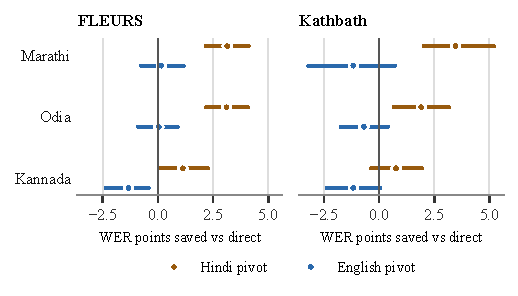
\includegraphics[width=\columnwidth]{figures/fig_gains.pdf}
\caption{WER gain over direct fine-tuning. Points show the measured gain
and bars show 95\% paired-bootstrap intervals.}
\label{fig:gains}
\end{figure}

% Generated by report/paper/build_assets.py from results/. Do not edit numbers by hand.
\begin{table}[!t]
\caption{Transfer Gains in WER Points With 95\% Paired-Bootstrap Intervals. Positive Means Fewer Errors; $\Delta = G_{\mathrm{Hi}} - G_{\mathrm{En}}$; Bold: Interval Excludes Zero}
\label{tab:gains}
\centering\scriptsize
\setlength{\tabcolsep}{2.2pt}
\begin{tabular}{@{}llccc@{}}
\hline
Target & Test & $G_{\mathrm{Hi}}$ & $G_{\mathrm{En}}$ & $\Delta$\\
\hline
Marathi & FLEURS & \textbf{+3.1} [2.2, 4.1] & +0.2 [$-$0.8, 1.2] & \textbf{+3.0} [2.1, 3.9]\\
 & Kathbath & \textbf{+3.5} [2.0, 5.2] & $-$1.2 [$-$3.2, 0.7] & \textbf{+4.6} [3.3, 6.4]\\
\hline
Odia & FLEURS & \textbf{+3.1} [2.2, 4.1] & 0.0 [$-$0.9, 0.9] & \textbf{+3.1} [2.1, 4.0]\\
 & Kathbath & \textbf{+1.9} [0.7, 3.2] & $-$0.7 [$-$1.8, 0.4] & \textbf{+2.6} [1.4, 3.9]\\
\hline
Kannada & FLEURS & \textbf{+1.1} [0.1, 2.3] & \textbf{$-$1.3} [$-$2.4, $-$0.4] & \textbf{+2.5} [1.4, 3.5]\\
 & Kathbath & +0.8 [$-$0.4, 2.0] & $-$1.2 [$-$2.4, 0.1] & \textbf{+1.9} [0.7, 3.2]\\
\hline
\end{tabular}
\end{table}


\subsection{Indo-Aryan Versus Dravidian Targets}

Hindi enhances all three languages, including Kannada, which is part of the Dravidian language family. On FLEURS, no confidence interval for the differences between the Hindi-specific gains excludes zero, i.e., none of them is statistically significant. On Kathbath, the Hindi-specific gain for Marathi exceeds that of Kannada by 2.7 points (95\% CI: 1.0 to 4.8), and that of Odia by 2.0 points (95\% CI: 0.1 to 4.3); the difference between Kannada and Odia gains is not significant. One possible reason for the improvement of Kannada could be some phonetic or acoustic properties shared by Indian languages. However, these properties were not measured in the present study.

\subsection{Odia: Tokenizer Cost and the Borrowed Language Token}

The cost of tokenization is high for the Odia language in comparison with the other languages used in the experiment. This language utilizes around 3.09 tokens per letter and 17.6 tokens per word, while the other languages used the same metrics at 1.29 (for Hindi), 1.30 (Marathi) and 1.89 (Kannada). The output limitation is another practical problem: 202 out of 875 Odia FLEURS references (23.1\%) were too long to be decoded and were excluded from evaluation. After training, the WER scores become comparable: Bengali 74.5/64.9, Assamese 74.9/65.0 and Hindi 73.8/64.6 on FLEURS/Kathbath.

% Generated by report/paper/build_assets.py from results/. Do not edit numbers by hand.
\begin{table}[!t]
\caption{Tokenizer Cost (FLEURS References) and the Borrowed Language Token for Odia}
\label{tab:odia}
\centering\scriptsize
\setlength{\tabcolsep}{3.5pt}
\begin{tabular}{@{}lrrr@{}}
\hline
Language & Tokens/letter & Tokens/word & Too long (\%)\\
\hline
Hindi & 1.29 & 5.18 & 0.0\\
Marathi & 1.30 & 7.60 & 0.0\\
Kannada & 1.89 & 13.87 & 1.3\\
Odia & 3.09 & 17.64 & 23.1\\
\hline
\end{tabular}

\vspace{4pt}
\begin{tabular}{@{}lccc@{}}
\hline
 & Zero-shot WER & Odia script & Trained WER\\
Token & FLEURS / Kathbath & (\%) & FLEURS / Kathbath\\
\hline
\texttt{<|bn|>} & 194.2 / 184.2 & 0 $\rightarrow$ 100 & 74.5 / 64.9\\
\texttt{<|as|>} & 199.3 / 182.5 & 0 $\rightarrow$ 100 & 74.9 / 65.0\\
\texttt{<|hi|>} & 210.3 / 230.6 & 0 $\rightarrow$ 100 & 73.8 / 64.6\\
\hline
\end{tabular}
\end{table}


\subsection{Effect of the Scoring Rules}

Removing
punctuation through the normalizer used in this study lowers FLEURS WER
by roughly 4.7 to 8.4 points across the nine trained models. Kathbath
references contain no punctuation, so the raw and normalized scores are
nearly the same there. Whisper's BasicTextNormalizer gives much lower
values; for example, Marathi FLEURS WER changes from 60.3 to 30.5,
because that normalizer removes the vowel signs that are part of the
written forms of Indic words. Such a score should not be treated as a
fair measure of recognition quality. The Hindi-pivot model remains first
under the three scoring rules, although Whisper's normalizer changes the
ordering of the direct and English-pivot models in two of the six
comparisons.

\subsection{On-Device Deployment}

The FP16 models converted to MLX occupy about 143.7 MB and run with an
RTF between 0.032 and 0.059 on the Apple M4, which is comfortably faster
than real time. The 4-bit versions are smaller at about
42.2 MB, or roughly one-third of the FP16 size, but their WER is generally
6 to 13 points worse. The Kannada result is especially concerning:
its CER rises from 17.0 to 72.1 after quantization. Based on these
measurements, FP16 is the more reliable choice for deployment.

% Generated by report/paper/build_assets.py from results/. Do not edit numbers by hand.
\begin{table}[!t]
\caption{On-Device Deployment (MLX, Apple M4): 100 FLEURS Clips per Model. RTF = Decoding Time / Audio Duration}
\label{tab:deploy}
\centering\scriptsize
\setlength{\tabcolsep}{3.4pt}
\begin{tabular}{@{}llrrrrr@{}}
\hline
Model & Weights & MB & RTF & WER & CER & WER (PyTorch)\\
\hline
Hindi pivot & fp16 & 144 & 0.032 & 41.1 & 15.5 & 41.7\\
 & 4-bit & 42 & 0.022 & 47.7 & 19.5 & \\
Hi$\rightarrow$Mr & fp16 & 144 & 0.038 & 64.7 & 21.1 & 63.2\\
 & 4-bit & 42 & 0.025 & 70.8 & 24.0 & \\
Hi$\rightarrow$Or & fp16 & 144 & 0.059 & 72.0 & 27.0 & 71.7\\
 & 4-bit & 42 & 0.044 & 78.5 & 31.8 & \\
Hi$\rightarrow$Kn & fp16 & 144 & 0.058 & 66.9 & 17.0 & 64.4\\
 & 4-bit & 42 & 0.058 & 79.9 & 72.1 & \\
\hline
\end{tabular}
\end{table}


\subsection{Limitations}

Each configuration used one training seed, so the bootstrap intervals capture variation in the test samples, not variation between independent training runs. We used Whisper-base and seeded subsets of two test datasets, and the large number of Odia references that exceed the decoder limit means that the Odia scores describe only the references the model could produce. Like Hindi, Marathi also uses the Devanagari script, making it difficult to separate script effects from family effects. Lastly, the intended native speakers' listening notes and error sheets were not available in time for analysis; hence, we cannot state what error classes the Hindi pivot sorted out.

% ======================================================================
\section{Conclusion and Future Scope}

This study compares direct fine-tuning with two-stage adaptation via Hindi and English for Marathi, Odia and Kannada. It was found that Hindi had a positive impact on WER for all three languages, whilst English did not produce any significant improvements given the same 45-hour pivot budget. This is important, as we can see that there are benefits to using Hindi as a pivot for languages outside of Indo-Aryan (Kannada). Due to inconsistencies at the family level between FLEURS and Kathbath, and the differences in domains for the recordings and the model's existing familiarity with the language for the English control, it cannot be said that the improvements are purely due to linguistic relatedness.

There are many clear improvements to be made. Firstly, a Dravidian pivot such as Tamil or Telugu could be used to test for transfer in the opposite direction, and the addition of Marathi-to-Odia and Kannada-to-Odia runs would increase the comparisons made for Odia. More training seeds should also be used alongside larger Whisper models to see how consistent the improvements are. In future, it would be good to have an experiment that isolates the effect of script similarities versus family similarities, and to look at different tokenizers which represent Odia more efficiently. Listening notes from native speakers and complete error sheets should also be included so that the paper can state what types of errors were corrected.

% ======================================================================
% References are numbered in order of first citation (IEEE style).
\begin{thebibliography}{24}

\bibitem{conneau2021xlsr}
A. Conneau, A. Baevski, R. Collobert, A. Mohamed, and M. Auli,
``Unsupervised Cross-Lingual Representation Learning for Speech
Recognition,'' in \emph{Proc. INTERSPEECH}, 2021, pp. 2426--2430.

\bibitem{babu2022xlsr}
A. Babu, C. Wang, A. Tjandra, K. Lakhotia, Q. Xu, N. Goyal,
K. Singh, P. von Platen, Y. Saraf, J. Pino, A. Baevski, A. Conneau, and
M. Auli, ``XLS-R: Self-Supervised Cross-Lingual Speech Representation
Learning at Scale,'' in \emph{Proc. INTERSPEECH}, 2022, pp. 2278--2282.

\bibitem{radford2023whisper}
A. Radford, J. W. Kim, T. Xu, G. Brockman, C. McLeavey, and
I. Sutskever, ``Robust Speech Recognition via Large-Scale Weak
Supervision,'' in \emph{Proc. International Conference on Machine
Learning (ICML)}, 2023, pp. 28492--28518.

\bibitem{pratap2024mms}
V. Pratap, A. Tjandra, B. Shi, P. Tomasello, A. Babu, S. Kundu,
A. Elkahky, Z. Ni, A. Vyas, M. Fazel-Zarandi, A. Baevski, Y. Adi,
X. Zhang, W.-N. Hsu, A. Conneau, and M. Auli, ``Scaling Speech
Technology to 1{,}000+ Languages,'' \emph{Journal of Machine Learning
Research}, vol. 25, no. 97, pp. 1--52, 2024.

\bibitem{pillai2026multistage}
L. G. Pillai, K. Manohar, B. K. Raju, and E. Sherly, ``Multistage
Fine-tuning Strategies for Automatic Speech Recognition in Low-resource
Languages,'' \emph{ACM Transactions on Asian and Low-Resource Language
Information Processing}, vol. 25, no. 8, pp. 1--12, 2026,
doi: 10.1145/3813800.

\bibitem{rouditchenko2023unseen}
A. Rouditchenko, S. Khurana, S. Thomas, R. Feris, L. Karlinsky,
H. Kuehne, D. Harwath, B. Kingsbury, and J. Glass, ``Comparison of
Multilingual Self-Supervised and Weakly-Supervised Speech Pre-Training
for Adaptation to Unseen Languages,'' in \emph{Proc. INTERSPEECH}, 2023,
pp. 2268--2272.

\bibitem{song2024lorawhisper}
Z. Song, J. Zhuo, Y. Yang, Z. Ma, S. Zhang, and X. Chen, ``LoRA-Whisper:
Parameter-Efficient and Extensible Multilingual ASR,'' in \emph{Proc.
INTERSPEECH}, 2024, pp. 3934--3938.

\bibitem{hu2022lora}
E. J. Hu, Y. Shen, P. Wallis, Z. Allen-Zhu, Y. Li, S. Wang, L. Wang, and
W. Chen, ``LoRA: Low-Rank Adaptation of Large Language Models,'' in
\emph{Proc. International Conference on Learning Representations
(ICLR)}, 2022.

\bibitem{xu2024rehearsalfree}
T. Xu, K. Huang, P. Guo, Y. Zhou, L. Huang, H. Xue, and L. Xie,
``Towards Rehearsal-Free Multilingual ASR: A LoRA-Based Case Study on
Whisper,'' in \emph{Proc. INTERSPEECH}, 2024, pp. 2534--2538.

\bibitem{ferraz2024distilwhisper}
T. P. Ferraz, M. Z. Boito, C. Brun, and V. Nikoulina, ``Multilingual
DistilWhisper: Efficient Distillation of Multi-Task Speech Models via
Language-Specific Experts,'' in \emph{Proc. IEEE International
Conference on Acoustics, Speech and Signal Processing (ICASSP)}, 2024,
pp. 10716--10720.

\bibitem{houlsby2019adapters}
N. Houlsby, A. Giurgiu, S. Jastrzebski, B. Morrone, Q. de Laroussilhe,
A. Gesmundo, M. Attariyan, and S. Gelly, ``Parameter-Efficient Transfer
Learning for NLP,'' in \emph{Proc. International Conference on Machine
Learning (ICML)}, 2019, pp. 2790--2799.

\bibitem{pfeiffer2020madx}
J. Pfeiffer, I. Vuli\'{c}, I. Gurevych, and S. Ruder, ``MAD-X: An
Adapter-Based Framework for Multi-Task Cross-Lingual Transfer,'' in
\emph{Proc. Empirical Methods in Natural Language Processing (EMNLP)},
2020, pp. 7654--7673.

\bibitem{javed2024indicvoices}
T. Javed, J. Nawale, E. George, S. Joshi, K. Bhogale, D. Mehendale,
I. Sethi, \emph{et al.},
``IndicVoices: Towards Building an Inclusive Multilingual Speech Dataset
for Indian Languages,'' in \emph{Findings of the Association for
Computational Linguistics: ACL}, 2024, pp. 10740--10782.

\bibitem{javed2023indicsuperb}
T. Javed, K. S. Bhogale, A. Raman, P. Kumar, A. Kunchukuttan, and
M. M. Khapra, ``IndicSUPERB: A Speech Processing Universal Performance
Benchmark for Indian Languages,'' in \emph{Proc. AAAI Conference on
Artificial Intelligence}, vol. 37, no. 11, 2023, pp. 12942--12950.

\bibitem{bhogale2023vistaar}
K. S. Bhogale, S. Sundaresan, A. Raman, T. Javed, M. M. Khapra, and
P. Kumar, ``Vistaar: Diverse Benchmarks and Training Sets for Indian
Language ASR,'' in \emph{Proc. INTERSPEECH}, 2023, pp. 4384--4388.

\bibitem{conneau2023fleurs}
A. Conneau, M. Ma, S. Khanuja, Y. Zhang, V. Axelrod, S. Dalmia,
J. Riesa, C. Rivera, and A. Bapna, ``FLEURS: Few-Shot Learning
Evaluation of Universal Representations of Speech,'' in \emph{Proc. IEEE
Spoken Language Technology Workshop (SLT)}, 2023, pp. 798--805.

\bibitem{pineiro2024weighted}
A. Pi\~{n}eiro-Mart\'{i}n, C. Garc\'{i}a-Mateo, L. Doc\'{i}o-Fern\'{a}ndez,
M. del Carmen L\'{o}pez-P\'{e}rez, and G. Rehm, ``Weighted
Cross-Entropy for Low-Resource Languages in Multilingual Speech
Recognition,'' in \emph{Proc. INTERSPEECH}, 2024, pp. 1235--1239.

\bibitem{panayotov2015librispeech}
V. Panayotov, G. Chen, D. Povey, and S. Khudanpur, ``Librispeech: An
ASR Corpus Based on Public Domain Audio Books,'' in \emph{Proc. IEEE
International Conference on Acoustics, Speech and Signal Processing
(ICASSP)}, 2015, pp. 5206--5210.

\bibitem{ardila2020commonvoice}
R. Ardila, M. Branson, K. Davis, M. Kohler, J. Meyer, M. Henretty,
R. Morais, L. Saunders, F. M. Tyers, and G. Weber, ``Common Voice: A
Massively-Multilingual Speech Corpus,'' in \emph{Proc. Language
Resources and Evaluation Conference (LREC)}, 2020, pp. 4218--4222.

\bibitem{wolf2020transformers}
T. Wolf, L. Debut, V. Sanh, J. Chaumond, C. Delangue, A. Moi,
P. Cistac, T. Rault, R. Louf, M. Funtowicz, \emph{et al.},
``Transformers: State-of-the-Art Natural Language Processing,'' in
\emph{Proc. EMNLP: System Demonstrations}, 2020, pp. 38--45.

\bibitem{peft2022}
S. Mangrulkar, S. Gugger, L. Debut, Y. Belkada, S. Paul, B. Bossan, and
M. Tietz, ``PEFT: State-of-the-Art Parameter-Efficient Fine-Tuning
Methods,'' 2022. [Online]. Available: \url{https://github.com/huggingface/peft}

\bibitem{bisani2004bootstrap}
M. Bisani and H. Ney, ``Bootstrap Estimates for Confidence Intervals in
ASR Performance Evaluation,'' in \emph{Proc. IEEE International
Conference on Acoustics, Speech and Signal Processing (ICASSP)}, vol. 1,
2004, pp. I-409--I-412.

\bibitem{mlx2023}
A. Hannun, J. Digani, A. Katharopoulos, and R. Collobert, ``MLX:
Efficient and Flexible Machine Learning on Apple Silicon,'' 2023.
[Online]. Available: \url{https://github.com/ml-explore/mlx}

\end{thebibliography}

\end{document}
